\documentclass[11pt]{article}
\usepackage[margin=1in]{geometry}
\usepackage{graphicx}
\usepackage{amsmath,amssymb}
\usepackage{booktabs}
\usepackage{caption}
\usepackage[hidelinks]{hyperref}
\usepackage{parskip}

\title{\textbf{CSc 8830 Computer Vision, Module 4}\\[2pt]
Finding the Boundary of a Human in RGB and Thermal Images\\
with Classical Computer Vision}
\author{Sirichandana Bikkasani \\ Georgia State University}
\date{\today}

\begin{document}
\maketitle

\begin{abstract}
This module outlines a person in a normal colour (RGB) image and in a thermal
(infrared) image using classical OpenCV only. The segmentation uses
thresholding, morphology, connected components, contours and GrabCut, with no
deep learning or machine learning. Each result is then placed next to SAM2 (the
Segment Anything Model 2), the reference the assignment asks us to compare against.
Section~\ref{sec:theory} works through, with derivations, how edge detection and
region segmentation can be done in the Fourier (frequency) domain. A Streamlit
web application makes every part reachable and lets the reader run the methods on
their own images.

\smallskip
\noindent\textbf{Live web app:} \url{https://csc8830-module4-human-seg.streamlit.app}\\
\textbf{Code repository:} \url{https://github.com/siri423/CSc8830-Computer-Vision}
\end{abstract}

\section{Where each requirement is covered}
\begin{center}
\begin{tabular}{ll}
\toprule
\textbf{Requirement} & \textbf{Where} \\
\midrule
Q1, human boundary in an RGB image (classical) & \texttt{src/rgb\_segment.py}, app tab RGB \\
Q2, human boundary in a thermal image (classical) & \texttt{src/thermal\_segment.py}, app tab Thermal \\
Comparison with SAM2 & \texttt{src/compare.py}, Section~\ref{sec:compare}, app tab Compare \\
Q3, Fourier theory for edges and regions & Section~\ref{sec:theory}, \texttt{src/fourier.py}, app tab Theory \\
Web application demo & \texttt{app.py} (Streamlit) \\
\bottomrule
\end{tabular}
\end{center}

\section{Q1: Human boundary in an RGB image}
In a colour photo the person and the background mainly differ in colour, so we
use GrabCut~\cite{grabcut}. GrabCut fits Gaussian mixtures to the foreground and
background colours and cuts the lowest cost boundary between them. It learns
those colour statistics from this one image, so it is not a trained model.

The steps are as follows. First we build an automatic seed, called a trimap: a
thin outer border is marked as sure background, a central column as probable
foreground, and a core torso block as sure foreground, so no clicking is needed.
The sure foreground core is what keeps parts whose colour matches the background,
such as hair against a beige backdrop, from being removed. Then we run GrabCut.
Next we clean the mask with a morphological opening to drop speckle and a closing
to fill small gaps, keep the single largest connected component since a person is
one object, and fill interior holes. Finally we trace the outer contour, which is
the boundary we report.

\begin{figure}[h]
\centering
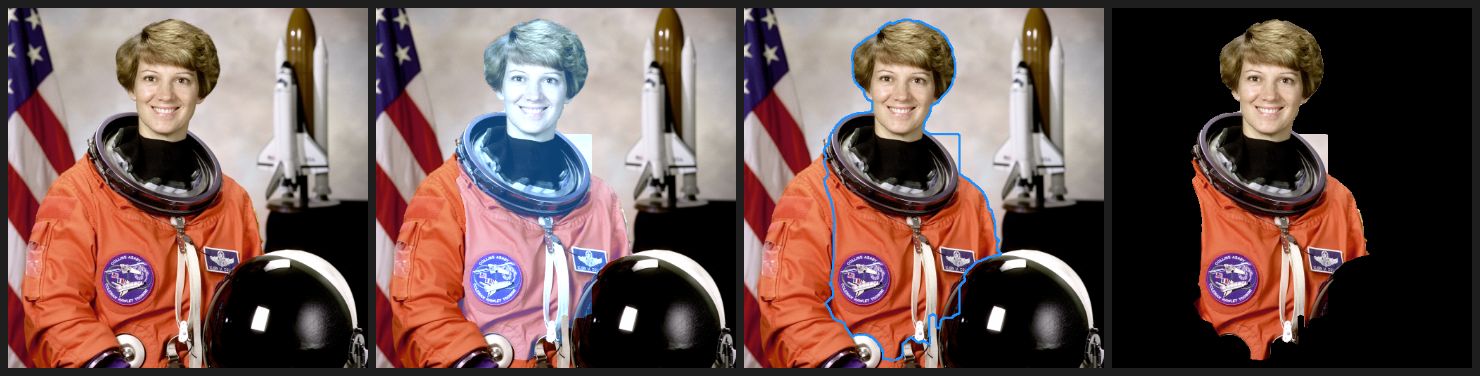
\includegraphics[width=\linewidth]{outputs/rgb_panel.png}
\caption{RGB result. From left to right: input, shaded mask, boundary, and the
image with the background removed. GrabCut captures the head, face and suit and
leaves out the flag, the shuttle model and the black helmet.}
\end{figure}

\section{Q2: Human boundary in a thermal image}
In a thermal image a warm body radiates more than the cool ground, so the person
is a bright, compact, roughly vertical blob. Colour models are not needed;
intensity and shape are enough. The one difficulty is that other things are hot
too, such as sunlit walls and lit windows, so the brightest pixel is not always
the person. We handle this with a two stage, coarse to fine method.

Stage one locates the person. We blur to reduce sensor noise, threshold at the
larger of the Otsu value and a high intensity percentile so only the hottest
regions remain, and clean up with morphology. Then we score every hot blob on how
human it looks, using shape and context only: an aspect ratio near two to one
(an upright person rather than a thin window), a ground plane prior (people stand
low in the frame, not high on a building), isolation (a person is ringed by cool
ground, whereas a window sits inside a warm wall), and size and solidity. The
best scoring blob is the person.

Stage two refines the outline. We crop a box around the located person, extended
downward so the dimmer legs are included, and run a local Otsu threshold inside
it. Because that box leaves out the far away hot windows, a lower local threshold
safely recovers the whole body. We then fill holes and trace the contour.

\begin{figure}[h]
\centering
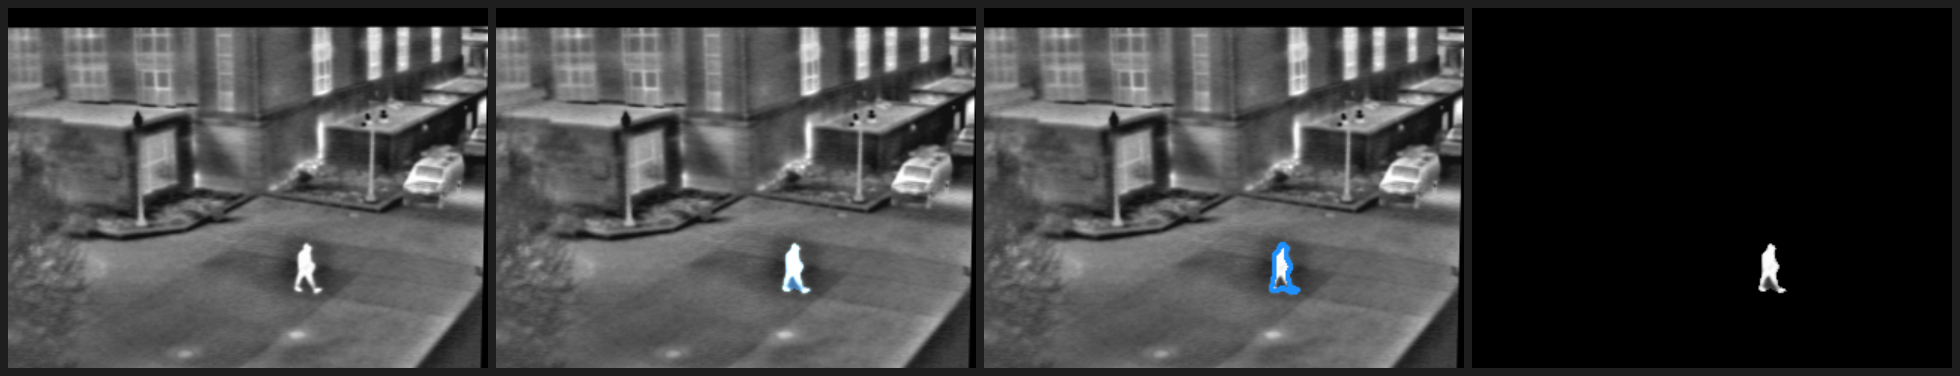
\includegraphics[width=\linewidth]{outputs/thermal_panel.png}
\caption{Thermal result. From left to right: input, shaded mask, boundary, and
the background removed image. The pedestrian is outlined from head to feet while
the warm building windows are ignored.}
\end{figure}

\section{Comparison with SAM2}\label{sec:compare}
We compare each classical mask against SAM2, the Segment Anything Model 2. We run
SAM2 through its image predictor demo and prompt it with a single foreground point
on the person. SAM2 is used only as the reference; our own code never uses it. We report three numbers: the Intersection over Union (IoU, Jaccard), the
Dice coefficient (F1), and a boundary F-score that matches the two outlines
within a two pixel tolerance. The boundary F-score is the one that speaks
directly to exact boundary quality.

\begin{table}[h]
\centering
\begin{tabular}{lccc}
\toprule
\textbf{Image} & \textbf{IoU} & \textbf{Dice} & \textbf{Boundary-F @2px} \\
\midrule
RGB (astronaut)      & 0.65 & 0.79 & 0.33 \\
Thermal (pedestrian) & 0.76 & 0.86 & 0.96 \\
\bottomrule
\end{tabular}
\caption{Agreement of our classical masks with SAM2.}
\end{table}

\begin{figure}[h]
\centering
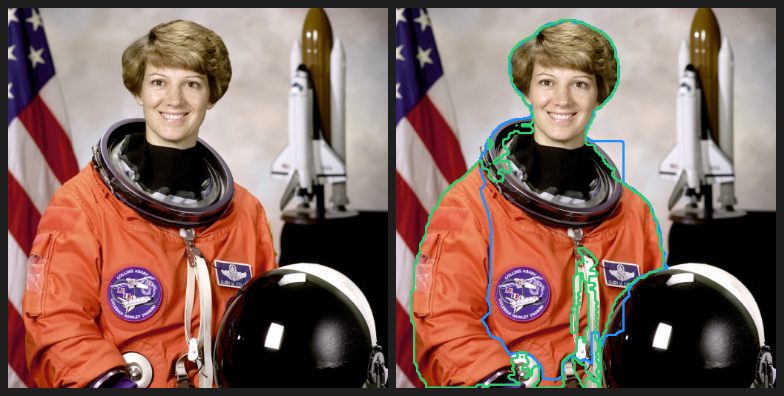
\includegraphics[width=\linewidth]{outputs/rgb_compare.png}\\[4pt]
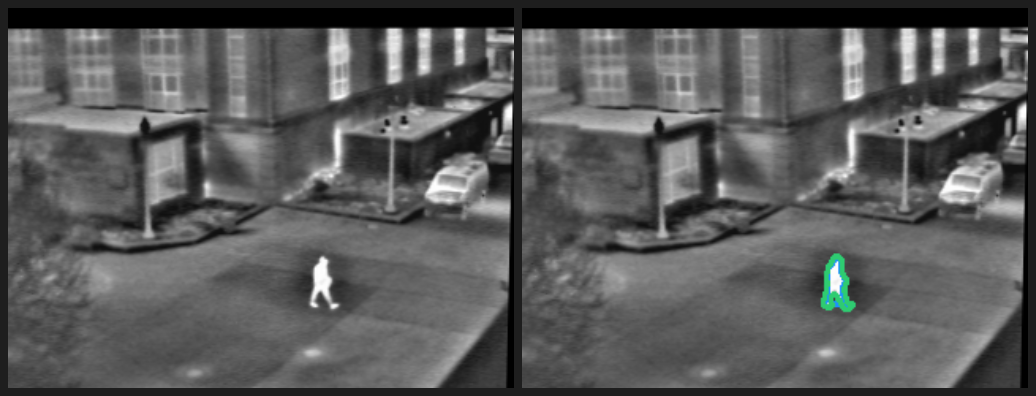
\includegraphics[width=\linewidth]{outputs/thermal_compare.png}
\caption{Blue is our classical boundary, green is SAM2. Top row is the RGB image,
bottom row is the thermal image.}
\end{figure}

On the thermal image the classical pipeline almost matches SAM2, with an IoU of
$0.76$ and a boundary F-score of $0.96$. A warm body against a cool background is
a high contrast case that thresholding handles well. On the RGB image the
classical result is weaker, with an IoU of $0.65$ and a boundary F-score of
$0.33$. GrabCut recovers the person as a whole, but where foreground and
background colours are similar, such as hair against the beige backdrop or the
arm against the suit, its boundary drifts, while SAM2 tracks the true edge. This
is the trade off the exercise is about: classical methods are simple and need no
training, while a learned model like SAM2 follows hard boundaries that colour or
intensity cues alone cannot resolve.

\section{Q3: Edge detection and region segmentation in the Fourier domain}
\label{sec:theory}
\textbf{The transform.} For an image $f(x,y)$ the two dimensional Fourier
transform is
\begin{equation}
F(u,v)=\iint_{-\infty}^{\infty} f(x,y)\,e^{-j2\pi(ux+vy)}\,dx\,dy,
\end{equation}
with inverse $f(x,y)=\iint F(u,v)\,e^{\,j2\pi(ux+vy)}\,du\,dv$. Slowly varying,
smooth regions concentrate their energy at low frequencies (small
$D=\sqrt{u^2+v^2}$), while sharp changes, which is what edges and fine texture
are, contribute high frequencies (large $D$).

\subsection{Edge detection is high-pass filtering}
Edges are places where $f$ changes fast, meaning large derivatives. The
derivative theorem of the Fourier transform says
\begin{equation}
\mathcal{F}\!\left\{\frac{\partial f}{\partial x}\right\}=j2\pi u\,F(u,v),
\qquad
\mathcal{F}\!\left\{\frac{\partial f}{\partial y}\right\}=j2\pi v\,F(u,v).
\end{equation}
Taking a derivative multiplies the spectrum by a factor proportional to
frequency, so it lifts high frequencies and holds down low ones. Every gradient
based edge operator is therefore a high-pass filter. For the Laplacian
$\nabla^2 f=\partial^2 f/\partial x^2+\partial^2 f/\partial y^2$,
\begin{equation}
\mathcal{F}\{\nabla^2 f\}=(j2\pi u)^2F+(j2\pi v)^2F
=-4\pi^2\,(u^2+v^2)\,F(u,v)=-4\pi^2 D^2\,F(u,v),
\label{eq:lap}
\end{equation}
so the Laplacian is the high-pass transfer function $H(u,v)=-4\pi^2D^2$. To find
edges we keep the high frequencies, for example with a Gaussian high-pass filter
\begin{equation}
H_{\text{hp}}(u,v)=1-e^{-D^2/(2D_0^2)},
\end{equation}
form $G(u,v)=F(u,v)\,H_{\text{hp}}(u,v)$, and inverse transform. This is valid
because of the convolution theorem: convolving the image with an edge kernel
$h(x,y)$ in space is the same as multiplying spectra in frequency,
\begin{equation}
g=f * h \;\;\Longleftrightarrow\;\; G(u,v)=F(u,v)\,H(u,v).
\end{equation}
So applying an edge filter and multiplying by $H(u,v)$ are the same operation.

\subsection{Laplacian of Gaussian, a band-pass edge detector}
Differentiation also lifts noise, which lives at high $D$, so we smooth first
with a Gaussian $g_\sigma$, whose transform is again a Gaussian,
$\mathcal{F}\{g_\sigma\}=e^{-2\pi^2\sigma^2D^2}$. Combining this with the
Laplacian in \eqref{eq:lap} gives the Laplacian of Gaussian (LoG) transfer
function
\begin{equation}
H_{\text{LoG}}(u,v)=-4\pi^2 D^2\,e^{-2\pi^2\sigma^2 D^2}.
\end{equation}
This is a band-pass filter. It is zero at $D=0$, rises to a peak, then decays, so
it keeps edge scale frequencies and rejects both the flat background and high
frequency noise. Edges are the zero crossings of
$\mathcal{F}^{-1}\{F\,H_{\text{LoG}}\}$, the Marr and Hildreth criterion. A step
edge becomes a positive then negative swing in the second derivative, and the
crossing between them marks the edge. The parameter $\sigma$ sets the scale of
the edges detected.

\subsection{Region segmentation through the frequency domain}
A uniform region is dominated by low frequencies. Multiplying by a Gaussian
low-pass filter
\begin{equation}
H_{\text{lp}}(u,v)=e^{-D^2/(2D_0^2)},\qquad
f_{\text{lp}}=\mathcal{F}^{-1}\{F\,H_{\text{lp}}\},
\end{equation}
removes texture and noise so each region becomes nearly flat, and then a global
threshold such as Otsu separates the regions. This is the same smoothing then
threshold idea used for the thermal image in Q2, now written as a spectral
multiplication. Since $H_{\text{hp}}=1-H_{\text{lp}}$, one transform gives both:
high-pass pulls out the boundaries between regions and low-pass pulls out the
smooth interior of regions, and a closed high-pass contour encloses a low-pass
region.

\textbf{Texture regions with a Gabor filter bank.} When regions differ by texture
rather than brightness, a single threshold fails, but different textures sit in
different parts of the spectrum. A Gabor filter is a Gaussian multiplied by a
complex exponential, $h(x,y)=g_\sigma(x,y)\,e^{\,j2\pi(u_0x+v_0y)}$, with the
transform
\begin{equation}
H(u,v)=e^{-2\pi^2\sigma^2\left[(u-u_0)^2+(v-v_0)^2\right]},
\end{equation}
a Gaussian window centred on frequency $(u_0,v_0)$. Each Gabor is a band-pass
filter that selects one orientation and scale. Filtering the image with a bank of
Gabors at several $(u_0,v_0)$ gives every pixel a vector of responses, a local
frequency signature. Pixels with similar signatures are grouped, by thresholding
or clustering, into texture regions. This is the frequency domain route to
segmenting regions that intensity alone cannot separate.

\begin{figure}[h]
\centering
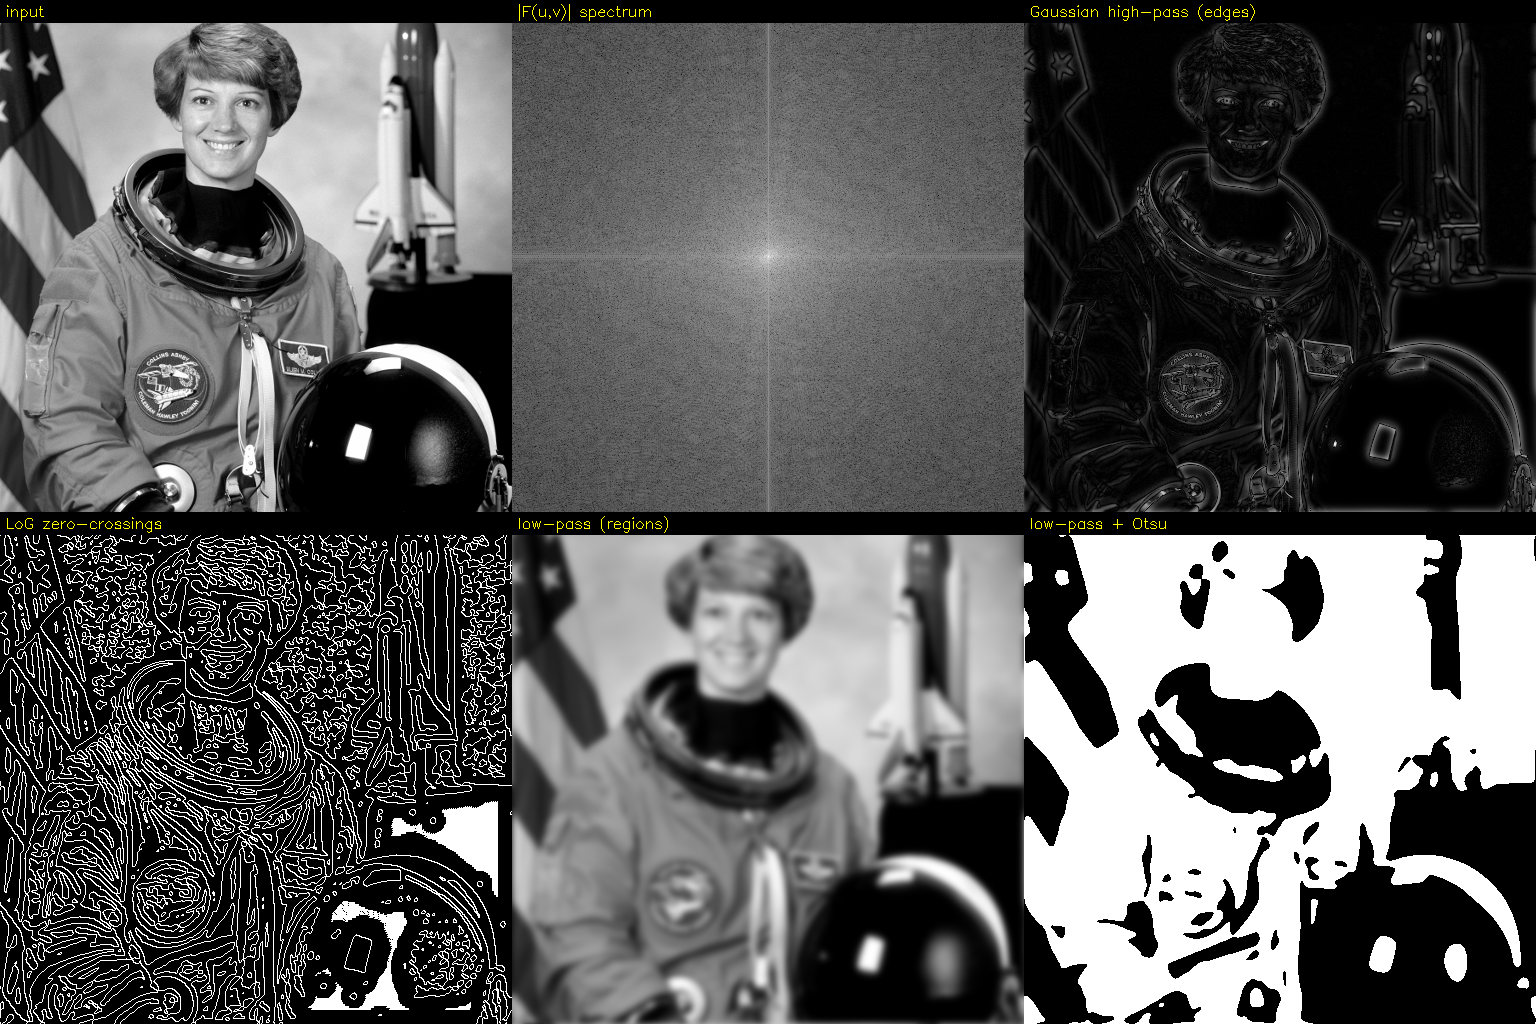
\includegraphics[width=\linewidth]{outputs/fourier_demo.png}
\caption{Frequency domain demonstration (\texttt{src/fourier.py}). Top row:
input, log magnitude spectrum $|F(u,v)|$, and a Gaussian high-pass result
(edges). Bottom row: LoG zero crossings, a Gaussian low-pass result (smoothed
regions), and low-pass followed by an Otsu threshold (region segmentation).}
\end{figure}

\section{How to run}
\begin{verbatim}
pip install -r requirements.txt
streamlit run app.py                 # web app (Q1, Q2, comparison, Q3 theory)

# or from the command line:
python -m src.rgb_segment      --image data/person_rgb.png
python -m src.thermal_segment  --image data/person_thermal.png
python -m src.compare
python -m src.fourier          --image data/person_rgb.png
\end{verbatim}

\textbf{Data.} RGB: the public domain \texttt{astronaut} image (NASA astronaut
Eileen Collins) from scikit-image. Thermal: a frame from the OSU Thermal
Pedestrian Database (OTCBVS Benchmark). \textbf{Note on SAM2.} SAM2 was run
through its public image predictor demo, prompted with a single foreground point
on the person, and the resulting mask was used as the reference. The exact steps
are in the README.

\begin{thebibliography}{9}
\bibitem{grabcut} C.\ Rother, V.\ Kolmogorov, A.\ Blake,
``GrabCut: interactive foreground extraction using iterated graph cuts,''
\emph{ACM SIGGRAPH}, 2004.
\bibitem{marr} D.\ Marr, E.\ Hildreth, ``Theory of edge detection,''
\emph{Proc.\ Royal Society of London B}, 1980.
\bibitem{gonzalez} R.\ C.\ Gonzalez, R.\ E.\ Woods,
\emph{Digital Image Processing}, Pearson (frequency domain filtering).
\bibitem{sam} A.\ Kirillov et al., ``Segment Anything,'' \emph{ICCV}, 2023;
N.\ Ravi et al., ``SAM 2: Segment Anything in Images and Videos,'' 2024.
\bibitem{osu} J.\ W.\ Davis, M.\ A.\ Keck, ``A two-stage template approach to
person detection in thermal imagery'' (OSU Thermal Pedestrian Database, OTCBVS
Benchmark), \emph{WACV}, 2005.
\end{thebibliography}

\end{document}
